\providecommand{\thebibpath}{..}
\makeatletter\def\input@path{{\thebibpath/}{.}}\makeatother
\documentclass[main.tex]{subfiles}
\begin{document}

\subsection{Changing platform}
\label{sec:platformio}

	The inherited embedded software required a toolchain called MPIDE (a fork of an early version of the Arduino IDE), which to quote the authors \enquote{is no longer being maintained, and is quickly falling behind}~\cite{ mpide}, as of January 2016. This is troublesome, as at some point in future, it may become impossible to download the software, which would make our embedded code unusable - better to deal with this technical debt now. The replacement software is an extension (\texttt{chipkit-core}) for the standard Arduino IDE.

	Unfortunately, this change in tools also comes with a change in hardware libraries.
	Due to license incompatibilities, the \texttt{plib} library bundled with MPIDE, which we were making use of to operate hardware registers, is not available in the Arduino IDE.
	This meant that large amounts of code that interfaced with hardware had to change. Many of these changes involves switching to the standard Arduino constructs for setting interrupts and writing pins.
	The rest required the use of features of the \texttt{chipkit-core} library.

	To verify that the transition was made correctly, some simple tests were performed with the motors, encoder, and accelerometer readings, all of which are easy to verify a log stream against by eye. One such mistake this picked up was that the encoders were no longer changing sign correctly.
	This was due to confusion\footnotemark between interrupt \emph{numbers} (referred to as \texttt{IRQ}s in the library) and interrupt \emph{vectors}.

	\footnotetext{A type of mistake that well-typed code written in C++, rather than C, would have prevented from happening in the first place. Alas, C is here to stay in the realm of embedded software libraries.}

	While the Arduino IDE family has the benefits of being widely-used, active, and open source, it has a bad approach to dependency management, which in practice makes it difficult to create small reusable components.
	To give an example, the following dependency structure is difficult for an Arduino project to handle:
	\begin{itemize}[noitemsep]
		\item The application depends on library \texttt{A} and \texttt{B}
		\item Library \texttt{B} depends on \texttt{C}
	\end{itemize}
	Worse yet, even if we remove the dependency on \texttt{C}, it is very difficult to distribute \texttt{A} alongside our application.

	There is a open source project that acknowledges and provides a solution to these shortcomings, PlatformIO~\cite{platformio}.
	This keeps the excellent cross-platform support that the Arduino libraries provide, and pairs them with a package manager, and a command line tool.
	One particularly useful feature is the ability to run unit tests on the Arduino, to verify the correctness of software.

\subsection{Building a communication interface}
	\label{sec:comms}

	In the review of the current system, we noted that the current system to configure the robot is manual and error prone.
	Echoing remarks by~\citeauthor{aleksi}~\cite[p.~34]{aleksi}, a worthwhile next step would be \enquote{automatically writing the policy parameters to the microcontroller program from Matlab as well as [adding] a direct serial communication between Matlab and the unicycle for data exchange}.

	The approach taken here unifies the above two suggestions.
	The goal is to have the program on the robot be static, and have it be reconfigurable over the serial link, as well as using that link to send back structured data.
	To achieve this, a communication protocol for sending structured messages must be designed. This breaks down into two parts:
	\begin{itemize}[noitemsep]
		\item Serialization (\enquote{structured}) -- converting an arbitrary data model into a series of bytes, and back again
		\item Framing (\enquote{messages}) -- distinguishing where one message begins and another ends
	\end{itemize}
	Both of these can be hard problems to get right, and so reinventing the wheel should be avoided.

	\subsubsection{Serialization}

		\begin{listingfloat}[t]
			\begin{lstlisting}[language=proto, gobble=6, frame=single]
			// Not shown: definitions of DebugLevel, LogBundle, and LogEntry
			syntax = "proto3";
			message DebugMessage {
				string s = 1;
				DebugLevel level = 2;
			}
			message RobotMessage {
				oneof msg {
					LogBundle log_bundle = 1;
					DebugMessage debug = 2;
					LogEntry single_log = 3;
				}
			}
			\end{lstlisting}
			\caption{A snippet of the protobuf description (\texttt{.proto} file) used with the robot}
			\label{lst:proto}
		\end{listingfloat}

		Google’s \enquote{Protocol Buffers}\cite{protobuf} (or simply \enquote{protobuf}) are a popular framework for implementing serialization, which are used extensively within Google, and have cross-language support.
		This framework requires a \texttt{.proto} file to be specified, like the one in \cref{lst:proto}.
		From this file, C++ and Python code can be generated to serialize and deserialize these messages into native types.

		An implementation of this for embedded C, with small code size and no heap allocation, exists as the Nanopb project~\cite{nanopb}, which thanks to our switch to PlatformIO \cref{sec:platformio}, is easy to include on our robot.
		Unfortunately, there is no first-party support of protobuf in Matlab, and the only available third-party implementation~\cite{protobuf-matlab} is difficult to install, and abandonware.\footnotemark

		\footnotetext{%
			The API of protobuf has changed significantly in the 5 years since this package was last modified.
			As such, were using protobuf from Matlab desired in future, the author would recommend starting the implementation from scratch as a protobuf python plugin, using the latest Google developer examples.
		}

	\subsubsection{Framing}

		It's worth recapping what level of abstraction the USB serial link exposes.
		Serial links allow a sequence of bytes to be sent one after another down a transmit (\texttt{tx}) channel, while at the same time a sequence of bytes are appear on the receive (\texttt{rx}) channel. The users of such a channel do not need to concern themselves with raw bits. There are two important properties to note here:
		\begin{itemize}[noitemsep]
			\item
				The receiver has to handle the byte as soon as it appears on the receive channel, as the channel has no memory.
				The typical approach is to add this byte to a queue or buffer, such that it can be processed later.
				This only delays the problem though -- this queue can become full, and subsequent bytes will be lost.
			\item
				Unlike I\textsuperscript{2}C, the channel provides no mechanism to group a set of bytes together.
				Every byte is sent separately, and in practice, implementations do not record at what time each byte was received (ruling out using a time delay to indicate \enquote{end-of-group}).
		\end{itemize}

		The problem of \enquote{framing}, then is build on this abstraction to provide a mechanism to group bytes together into packets. Consider the sequence of packets
		\enquote{\texttt{F1}\,\texttt{00}\,\texttt{D5}},
		\enquote{\texttt{0F}},
		\enquote{\texttt{C0}\,\texttt{FF}\,\texttt{EE}}, shown with each byte in hexadecimal notation.
		A na\"ive approach is to prefix a chunk of bytes by its length, giving
		\mbox{\enquote{%
			\textbf{\texttt{03}}\,\texttt{F1}\,\texttt{00}\,\texttt{D5}\,%
			\textbf{\texttt{01}}\,\texttt{0F}\,%
			\textbf{\texttt{03}}\,\texttt{C0}\,\texttt{FF}\,\texttt{EE}%
		}}, with inserted bytes shown in bold.
		To see why this is not enough, consider what happens if the\,\texttt{F1} byte does not fit in the buffer and is discarded. The receiver now sees \mbox{\enquote{%
			\textbf{\texttt{03}}\,\texttt{00}\,\texttt{D5}\,\texttt{01}\,%
			\textbf{\texttt{0F}}\,\texttt{03}\,\texttt{C0}\,\texttt{FF}\,\texttt{EE}\,%
			...%
		}} -- corruption in the first packet has corrupted the following two packets, and possibly the rest of the stream for all time!

		A good solution to this problem is COBS, which to quote the originating paper~\cite{cobs}, \enquote{allows new listeners to join a broadcast stream at any time and without fail receive and decode the very next error free packet} -- ideal for our scenario where the serial USB connection is plugged and unplugged (\cref{sec:untethered}). Under COBS, the example packets are encoded as
		\mbox{\enquote{%
			\textit{\texttt{02}}\,\texttt{F1}\,\textit{\texttt{02}}\,\texttt{D5}\,\textbf{\texttt{00}}\,%
			\textit{\texttt{02}}\,\texttt{0F}\,\textbf{\texttt{00}}\,%
			\textit{\texttt{04}}\,\texttt{C0}\,\texttt{FF}\,\texttt{EE}\,\textbf{\texttt{00}}%
		}}, with \textbf{\texttt{00}} bytes appear only at the end of each packet.
		The inserted italicized bytes encode zeros within packets by counting the number of bytes until the next zero.
		Using this method, dropping any non-zero byte will corrupt only a single packet, and dropping a zero byte will corrupt only two packets.

		Sadly, no implementation of COBS was available for the Arduino which was suitable for use with Nanopb\footnotemark.
		Messaging over serial is an essential part of many Arduino projects, and so the inability to assemble a robust messaging stack from library code is cause for alarm.
		In the interest of giving back to the community, the author published PacketIO~\cite{packetio}, a package to solve the framing problem.
		This package includes unit tests and online documentation, in order to help verify its correctness and encourage its use.

		\footnotetext{%
			A package implementing COBS for Arduino does exist, PacketSerial~\cite{packetserial}.
			However, this requires the entire message to be calculated before any of it is sent, whereas nanopb requires a streaming protocol. Nanopb's choice makes it able to write arbitrarily large messages piece by piece -- such as our state logs.
		}

	\subsubsection{Using the protocol}

		\begin{wrapfigure}[14]{R}{0.4\linewidth}
			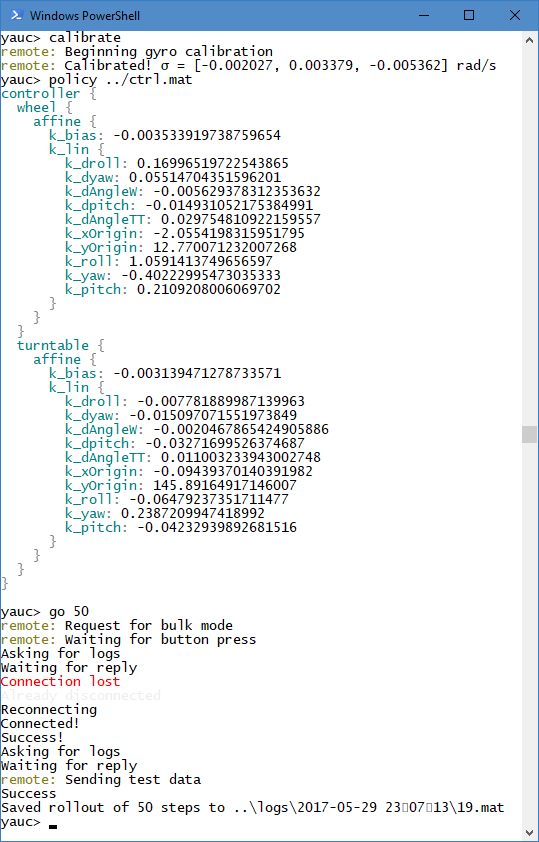
\includegraphics[width=\linewidth]{figures/cli.png}
			\caption{The CLI}
			\label{fig:cli}
		\end{wrapfigure}

		With a messaging interface on the robot, a tool was needed on the PC to communicate with it.
		Due to the previously-mentioned lack of protobuf implementation in Matlab, Python 3.5 was chosen as the tool for the job.

		For simplicity, the tool was created as an interactive command-line interface (CLI), rather than a graphical one.
		A screenshot of the interface is shown in \cref{fig:cli}.
		From this command line, commands can be sent to and data collected from the robot.
		Of particular note is that any diagnostic messages from the robot also appear in this interface, as they too go through the messaging interface. Example commands include:
		\begin{description}
			\item[\texttt{go} $\langle$n$\rangle$]
				Prepares for an n-timestep rollout. Once run, the robot can be detached, and the rollout begun. Upon reattaching the robot, the command line extracts the state logs, dumping them into a \texttt{.mat} file for the {\Pilco} Matlab code to read.
			\item[\texttt{policy}  $\langle$filename$\rangle$]
				Loads a policy from the provided \texttt{.mat} file onto the robot.
		\end{description}

		\begin{description}[topsep = \itemsep]
			\item[\texttt{calibrate}]
				Performs gyroscope recalibration -- this needs to be manually triggerable, so that the operator can ensure the robot is at rest.
		\end{description}

\subsection{Recovering and documenting pin assignments}
	\label{sec:pins}

	When adding the switch in \cref{sec:switch}, it was found to that no documentation was present on which pins were free and which ones were in use. It was decided that this would be easier to determine through reading the source code, rather than dismantling the electronics, and following traces.
	Unfortunately, the source code alone was not enough to reconstruct this, as some pins were not referred to by number, but by the hardware peripherals (timers, PWM, etc) they belong to, so the data sheet was needed too.

	The DRY principle (\cref{sec:dry}) stands against these mixed representations, so a novel system was invented to specify the pins numbers in the source code, but translate them into peripherals \emph{at compile time}.
	This is powerful, because it means that code which tries to use a pin for a peripheral it does not support \emph{will not compile}! The trick in the implementation is to exploit the \cpp{constexpr} keyword, and is shown in \cref{lst:constexpr}.
	Once this is done, the pins in use can be made directly readable from the source code, as in \cref{lst:pins}.

	\begin{listingfloat}
		\centering
		\begin{lstlisting}[language={[11]c++},gobble=6,frame=single]
			template<typename T>
			T failed(const char*) { while(1); }

			constexpr p32_timer& timer_for(uint8_t pin) {
				return pin == 4  ? tmr1 :
				       pin == 22 ? tmr3 :
				       pin == 23 ? tmr4 :
				       pin == 11 ? tmr5 :
				       failed<p32_timer&>("Timer does not exist");
			}

			constexpr p32_timer& ta = timer_for(4);  // ok, returns tmr1
			constexpr p32_timer& tb = timer_for(3);  // compiler error!
		\end{lstlisting}
		\caption{Compile-time pin-checking}
		\label{lst:constexpr}
		\medskip
		\small
		The last line is a compiler error because \cpp{failed} is not marked \cpp{constexpr}, which \enquote{contaminates} the \cpp{constexpr}-ness of \cpp{timer_for}, forbidding its result from being placed in \cpp{tb}.
	\end{listingfloat}

	\begin{listingfloat}[!tb]
		\begin{lstlisting}[language={[11]c++},gobble=6,frame=single]
			namespace pins {
				/** @name Encoders */
				static const uint8_t TT_DIR = 39;
				static const uint8_t W_DIR  = 47;
				static const uint8_t TT_CLK = 22;
				static const uint8_t W_CLK  = 23;
				/** @} */

				/** @name I2C Sensors */
				static const uint8_t IMU_SCL = 21;
				static const uint8_t IMU_SDA = 20;
				/** @} */

				/** @name Motors */
				static const uint8_t TT_FWD = 3;
				static const uint8_t TT_REV = 5;
				static const uint8_t W_FWD  = 6;
				static const uint8_t W_REV  = 9;
				/** @} */

				/** @name Human interaction */
				static const uint8_t SWITCH = 43;
				static const uint8_t LED    = PIN_LED1;
				static const uint8_t USB_RX = 0;
				static const uint8_t USB_TX = 1;
				/** @} */
			}
		\end{lstlisting}
		\caption{Pin assignments of the ChipKIT microcontroller}
		\label{lst:pins}
	\end{listingfloat}

\subsection{Measuring initial orientation}
\label{sec:acc:orient}
	Earlier work~\cite{aleksi} noted that there were issues with variation in orientation in which the robot is placed by the operator when started.
	This stems from the fact that the estimate of orientation used by the robot is from integration of angular velocity (\cref{sec:quat:int}), only giving a change in orientation -- yet the true dynamics depend on the absolute orientation with respect to gravity.
	In that work, there was discussion of learning these offsets and incorporating them into the dynamics model.
	While this would be a useful approach for building the dynamics model, it does not help in implementing a controller, as for this to work the embedded code would not only need to do the learning, but would need to do it online and in realtime.

	A better approach would be to simply measure the initial orientation, for which we already have a suitable sensor, the accelerometer. When the robot is not in motion, this measures only the acceleration due to gravity, telling us $\bm{a}$, the direction in which down lies in the frame of the robot.
	We know that for the upright robot, the reading of the accelerometer should be $\bm{a}_0 = \begin{bmatrix}0 & 0 & -g\end{bmatrix}^T$\footnotemark. We desire a quaternion (\cref{sec:quat:intro}) $\bm{q}$ that rotates $\bm{a}_0$ onto $\bm{a}$, from which it can be shown
	\footnotetext{%
		After the appropriate transformation from sensor to robot coordinates.
		We approximate this with a simple rotation matrix of
		$\left[\begin{smallmatrix}0 & 0 & -1 \\ 1 & 0 & 0 \\ 0 & -1 & 0\end{smallmatrix}\right]$.
		This is likely to be incorrect by the order of \SI{5}{\degree} on some axis, due to bending of components.
	}
	\begin{align}
		\bm{a} &= \bm{q}\bm{a}_0\bm{q}^*\, & \implies
		\bm{q}^2
			&= \operatorname{normalize}\left(
				\bm{a}_0 \cdot \bm{a} + \bm{a}_0 \times \bm{a}
			\right)
			\label{eq:quat-sqrt}
	\end{align}
	There are infinitely many solutions to this equation, lying on a circle in $\mathbb{H}$.
	We choose the rotation of minimum angle,
	\begin{align}
		\bm{q} &= \operatorname{normalize}(\bm{q}^2 + 1)\,, &
		%
		\parbox{\linewidth/5}{%
			\begin{tikzpicture}[
	trim axis left,
	trim axis right
]
	\begin{axis}[%
		width=\linewidth,
		height=7\linewidth/11,
		at={(0\linewidth,0\linewidth)},
		scale only axis,
		axis equal,
		axis lines=middle,
		xmin=-.2, xmax=2,
		ymin=-.2, ymax=1.2,
		xlabel=$w$,
		ylabel=$x$,
		xtick=\empty,
		ytick=\empty,
	]

	\draw[gray] (0,0) circle (1);

	\coordinate (q2p1) at (1.6, 0.8);
	\coordinate (q2) at (0.6, 0.8);
	\coordinate (one) at (1, 0);
	\coordinate (zero) at (0, 0);
	\coordinate (q) at (0.894427190999916, 0.447213595499958);

	\node[above, blue] at (q2) {\footnotesize $q^2$};
	\node[below right, red] at (one) {\footnotesize $1$};
	\node[above left, purple] at (q) {\footnotesize $q$};

	\draw[->, red, thick] (0,0) -- (one);
	\draw[->, blue, thick] (0,0) -- (q2);
	\draw[->, red, thick, dashed] (q2) -- (q2p1);
	\draw[->, blue, thick, dashed] (one) -- (q2p1);
	\draw[->, purple, thick] (0,0) -- (q);
	\draw[purple, thick, dashed] (q) -- (q2p1);

	\end{axis}
\end{tikzpicture}%

		}
	\end{align}
	for which the  graphical interpretation for the simplified case where $\bm{q}^2 = w + x\iu$ is shown on the right.

	The accelerometer does not tell us any information about the yaw angle (corresponding to the degree of freedom in \cref{eq:quat-sqrt}), so we are free to change the yaw rotation of the result as we please.
	Since our cost function penalizes yaw, it is sensible to choose $\psi = 0$.
	We can enforce this trivially by converting to Euler-YXZ angles, replacing $\psi$ with $0$, and converting back to a quaternion\footnotemark. The relevant conversions can be found in~\cite[eq~362 and 369]{diebel2006representing}, or in the embedded source code as \cpp{geometry::euler_angles<213>::operator quat()} and \cpp{geometry::euler_angles<213>::euler_angles<213>(quat q)}.

	\footnotetext{%
		In the source code, we take a more direct approach, noting that we need only extract the yaw from the quaternion, and post-multiply by a quaternion that removes that yaw.
		This approach removes the need to call any trigonometric functions.
	}

	With this change in place, the operator can worry less about the orientation in which the robot is released -- it now does not affect the correctness of the dynamics model, only the likelihood of falling over.
	This means that the operator too can learn that they are releasing in a bad position, as they are no longer constrained to releasing in the same way every time.


\subsection{Other improvements}
	Large amounts of additional refactoring not mentioned above happened within the embedded code, in order to try and comply better with DRY.
	Examples where code was duplicated (and subsequently fixed) include the:
	\begin{itemize}[noitemsep]
		\item handling of encoder signs -- once for each encoder.
		\item handling of motor operation -- once for each motor.
		\item conversion from imu sensor coordinates to robot coordinates -- once for each of the gyro and accelometer
		\item conversion from raw sensor reading to SI units -- conversion constants (or \enquote{magic numbers}) are duplicated throughout.
	\end{itemize}
	This is not an exhaustive list -- indeed, more problems are discovered during debugging later in this work.

\bib

\end{document}
